\chapter{Problem description }

The main objective was the assessment and improvement of some routines
used in the free energy package {\trafo}. A further goal was to
minimize the necessity of additional adjustments by the user, i.e.
reasonable mutation routes have to be generated automatically. The
proposed route should be directly usable for the further {\trafo}
workflow.

In a first step, the reliability of the current {\trafo} workflow
had to be assessed, for instance the quality of the proposed common
cores. Different settings for the construction of the maximum common
substructure were compared. 

The order of the transformation steps was optimized, especially
for the case of more complex mutation routes which occur for connected
dummy regions involving ring structures, multiple chains or different
atom types. 

Particularly intricate problems occur for ring structures. In contrast to a chain, which usually has only one possible mutation order without leading to disconnected components, multiple possible orders exist. (Because of this fact, the evaluation of the mutation algorithms in the following sections will focus on such transformations.) Neither should
the mutation of atoms generate vacancies in the inner part of the
molecule nor should opened rings remain longer than necessary and
a sufficiently systematic and - especially concerning rings - symmetric
processing of the nodes has to be performed. These rules have to be
implemented by maintaining the crucial constraint that no atoms are
detached from the main part encompassing the common core, i.e. no
disconnected components emerge under any circumstances.

Using a graph representation of the involved molecules, the construction
of the intermediates between the final states was optimized.
New algorithms have been written in Python and subsequently integrated
into the existing {\trafo} package. Finally, the effect of different
algorithms on the efficiency of the free energy calculations was validated by means of molecular dynamics simulations. 

To obtain a reliable test set of molecules, sdf-files of ligands were downloaded from the PDBbind-CN database. These test molecules should cover a
broad range in size, complexity and potentially intricate compounds,
like polycyclic structures and highly branched chains.

\section{Used algorithms and software packages}

The {\trafo} package is written in Python. Therefore, Python packages
also were used for molecule processing and graph representations.
The creation of molecule objects and the determination of the maximum
common substructure is done via Rdkit\cite{key-3}. NetworkX\cite{AricA.Hagberg.2008}
provides functions for graph visualization and analysis. It is easy to convert molecules created using Rdkit into NetworkX graph-objects
and hence utilize the functions of NetworkX for the molecules and
common cores constructed. Particularly, graph traversal algorithms
like breadth-first and depth-first search can be easily implemented
(see below).

\section{Assessment of common core settings}

Rdkit allows the search for a maximal common substructure (which can
serve as common core for {\trafo}) via the \texttt{rdFMCS.FindMCS}-function.
Per default, the objective is to maximize the number of atoms, albeit
different settings, like maximize the number of bonds or ignoring
or equalizing specific atom types are available. At the moment, for
{\trafo} maximization of atoms and atom identity is used. As stated above, the presence of hydrogens can influence
the maximum common substructure heavily (fig. 4.1) because the number of atoms is modified and this quantity is maximized for the maximal common substructure. 


Settings concerning the allowed involvement of ring structures in
the common core are of crucial importance. Firstly, these parameters
can influence the common core construction drastically and, secondly, they
can even be decisive whether the generated common core is valid for the
{\trafo} workflow.
Especially for the generation of common cores for polycyclic molecules, e.g. sterols, these parameters are of utmost importance.  
Important ring-related settings are \texttt{ringMatchesRingOnly}, \texttt{completeRingsOnly}
and the \texttt{ringCompare-parameter}. 

To obtain valid common cores of molecules involving cyclic structures for the processing of {\trafo}, \texttt{ringMatchesRingOnly}
and \texttt{completeRingsOnly} must be set to True: The former argument indicates
that ring atoms of one molecule are only matched against ring atoms
of the other molecule, the latter ensures that no partial rings are
involved in the common core. Especially the latter constraint is a
necessary condition for a valid common core. (Otherwise, if partial
rings take part of the common core, dummy regions will be inevitably
connected to the common core via multiple bonds.)

The \texttt{ringCompare}-parameter parameter accepts the \texttt{StrictRingFusion}-argument.
It imposes that in case of multiple rings aromaticity is properly
taken into account. Fig. 4.2 illustrates the effect of the parameters
on the common core of two cyclic example molecules. However, enforcing
of \texttt{StrictRingFusion} can still lead to maximum common substructures
that are not valid {\trafo} common cores in case of a dummy region
which is connected via multiple ring atoms of the same ring with the common
core. 
When an invalid common core is generated, it seems to be advisable to warn the user in this case that the common core does not fit the expectations of the {\trafo} workflow. 
The mutation algorithms presented below can deal with such invalid common cores. A helper function arbitrarily chooses one of the connections between common core and dummy region and the other ones are ignored for the mutation path. However, this only ensures that a mutation route is returned; the current {\trafo} workflow is not adapted to deal with such common cores in a proper way. Therefore it makes only sense for test purposes and is not a reasonable input for the regular workflow.
Alternatively, one could check after the creation if the common core is valid. If
it is not, one could for instance search for a new common core encompassing fewer
atoms until a valid common core is found (see below). A further option would be to prohibit the involvement of ring atoms for this particular molecule combination.

These problems occur because the requirements for a valid {\trafo} common core are more strict than the constraints imposed by rdkit  (even when all ring-related parameters are applied, i.e. \texttt{ringMatchesRingOnly}, \texttt{completeringsonly} and \texttt{strictringfusion}): For {\trafo}, is not only indispensable that the common core solely comprises complete rings, but also the molecule fragment consisting of the non-common core atoms (which implies that there is a unique connection between dummy region and common core).
An efficient and straightforward solution for this problem, which always yields the best - i.e. largest - valid common core if one exists, has been implemented:
The basic observation is that if common core atoms within a cyclic region give rise to a invalid common core, it is impossible that any atoms within this region could participate in a valid one (if this would be the case, the whole cyclic region would be already in the generated common core).
After generating a common core with standard parameters, it is checked if the additional requirements concerning the ring structure hold, i.e. if the non-common core atoms (as well as the common core atoms) of both molecules do not participate in a partial cycle.
(Alternatively, one could check if a path between the non-common core atoms adjacent to the common core, i.e. the X-atoms, exists. If this is the case, the common core obviously is not valid, since no unique atom which connects common core and a specific dummy region is present.)





\begin{figure}
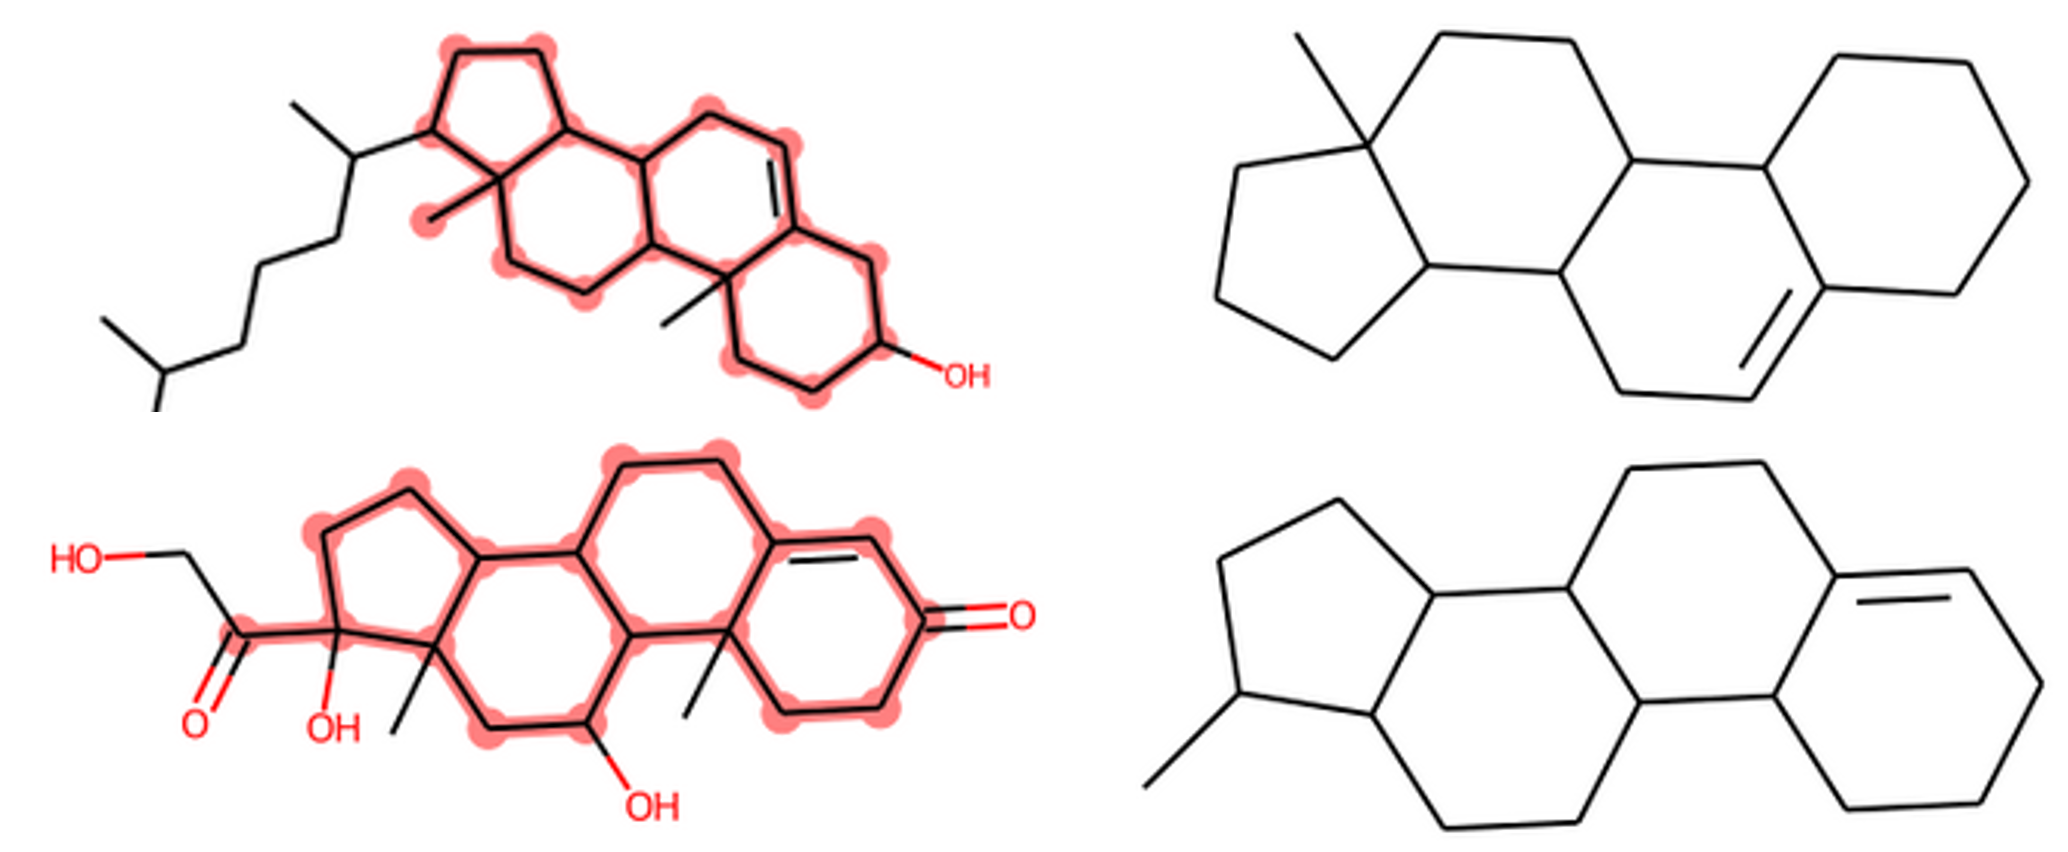
\includegraphics[scale=0.45]{sterols_wo_strictfusion}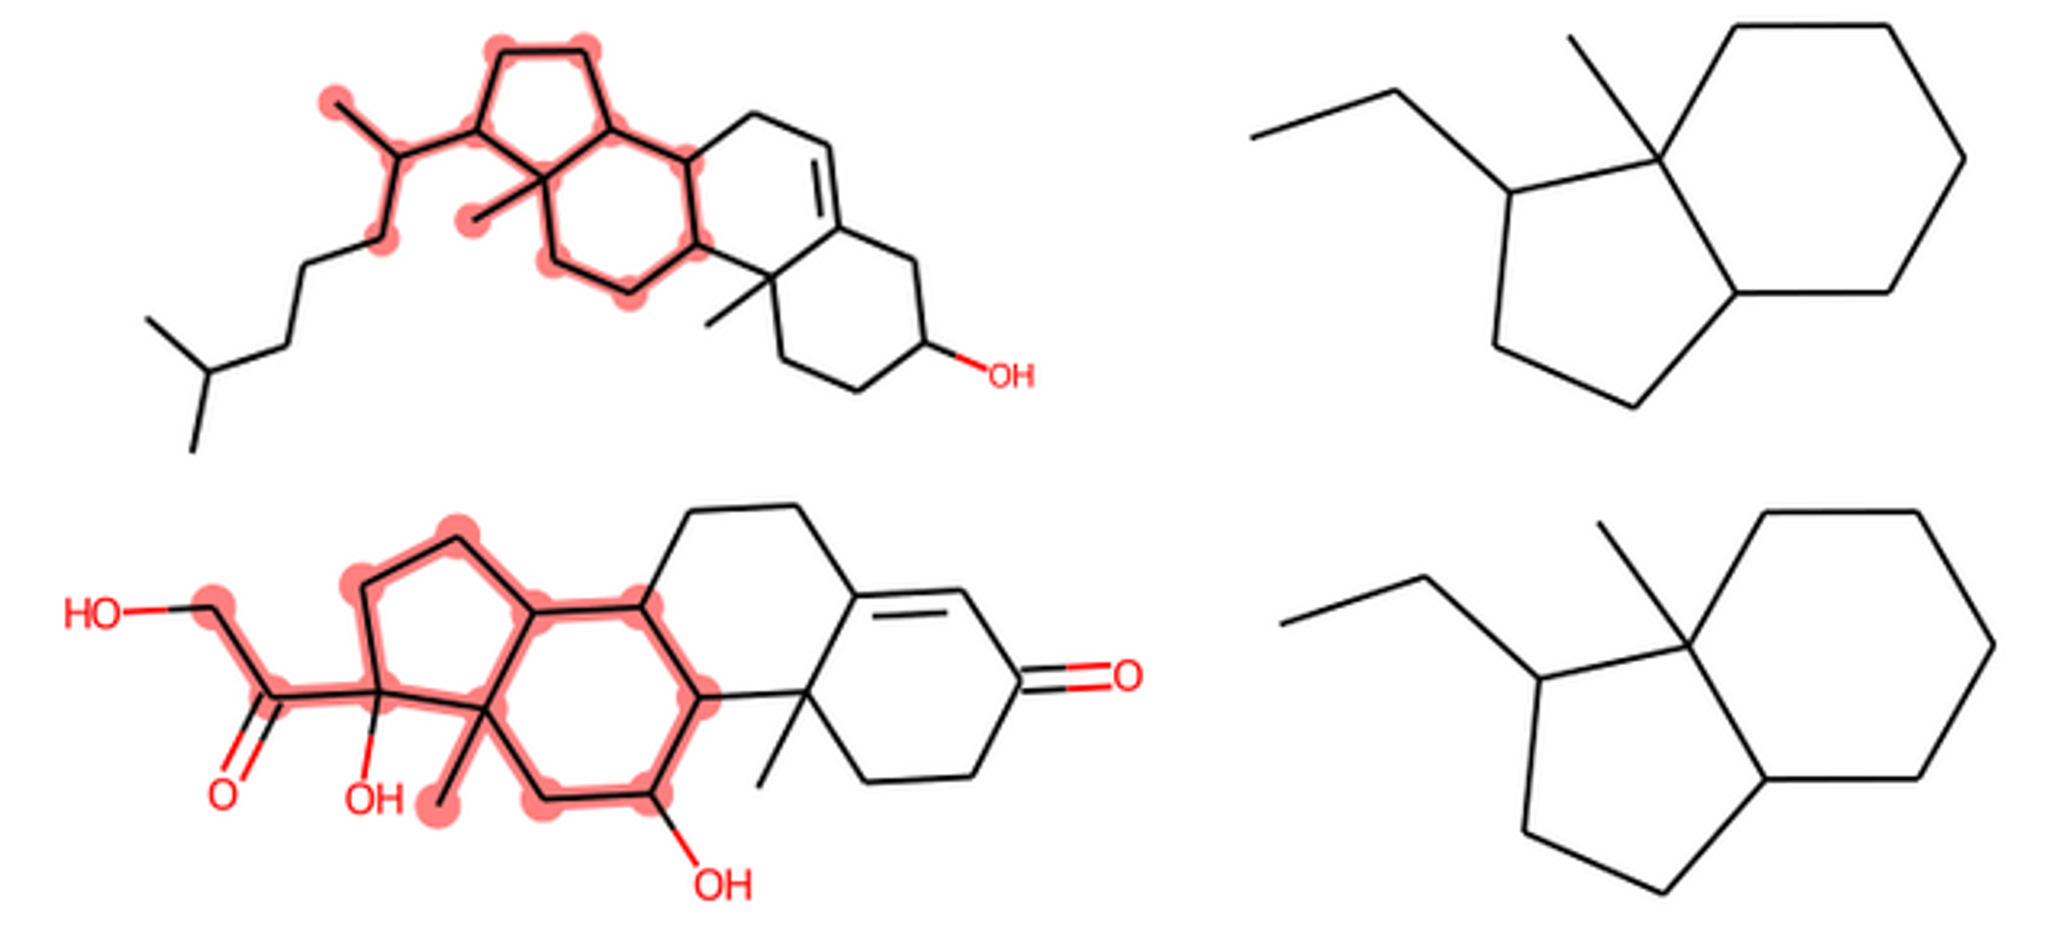
\includegraphics[scale=0.4]{sterols_w_strictfusion}

\caption{'Strict fusion' can affect the construction of the common core drastically; first and second column: Common core of two molecules (cholesterol
and cortisol) without strict fusion; third and fourth column: Common
core of two molecules with strict fusion; in the images of the full molecule graph common cores are marked in red. In this case, none of the settings yield a valid common core, the iterative approach explained in the main text would be necessary to obtain one. }

\end{figure}




\begin{figure}
	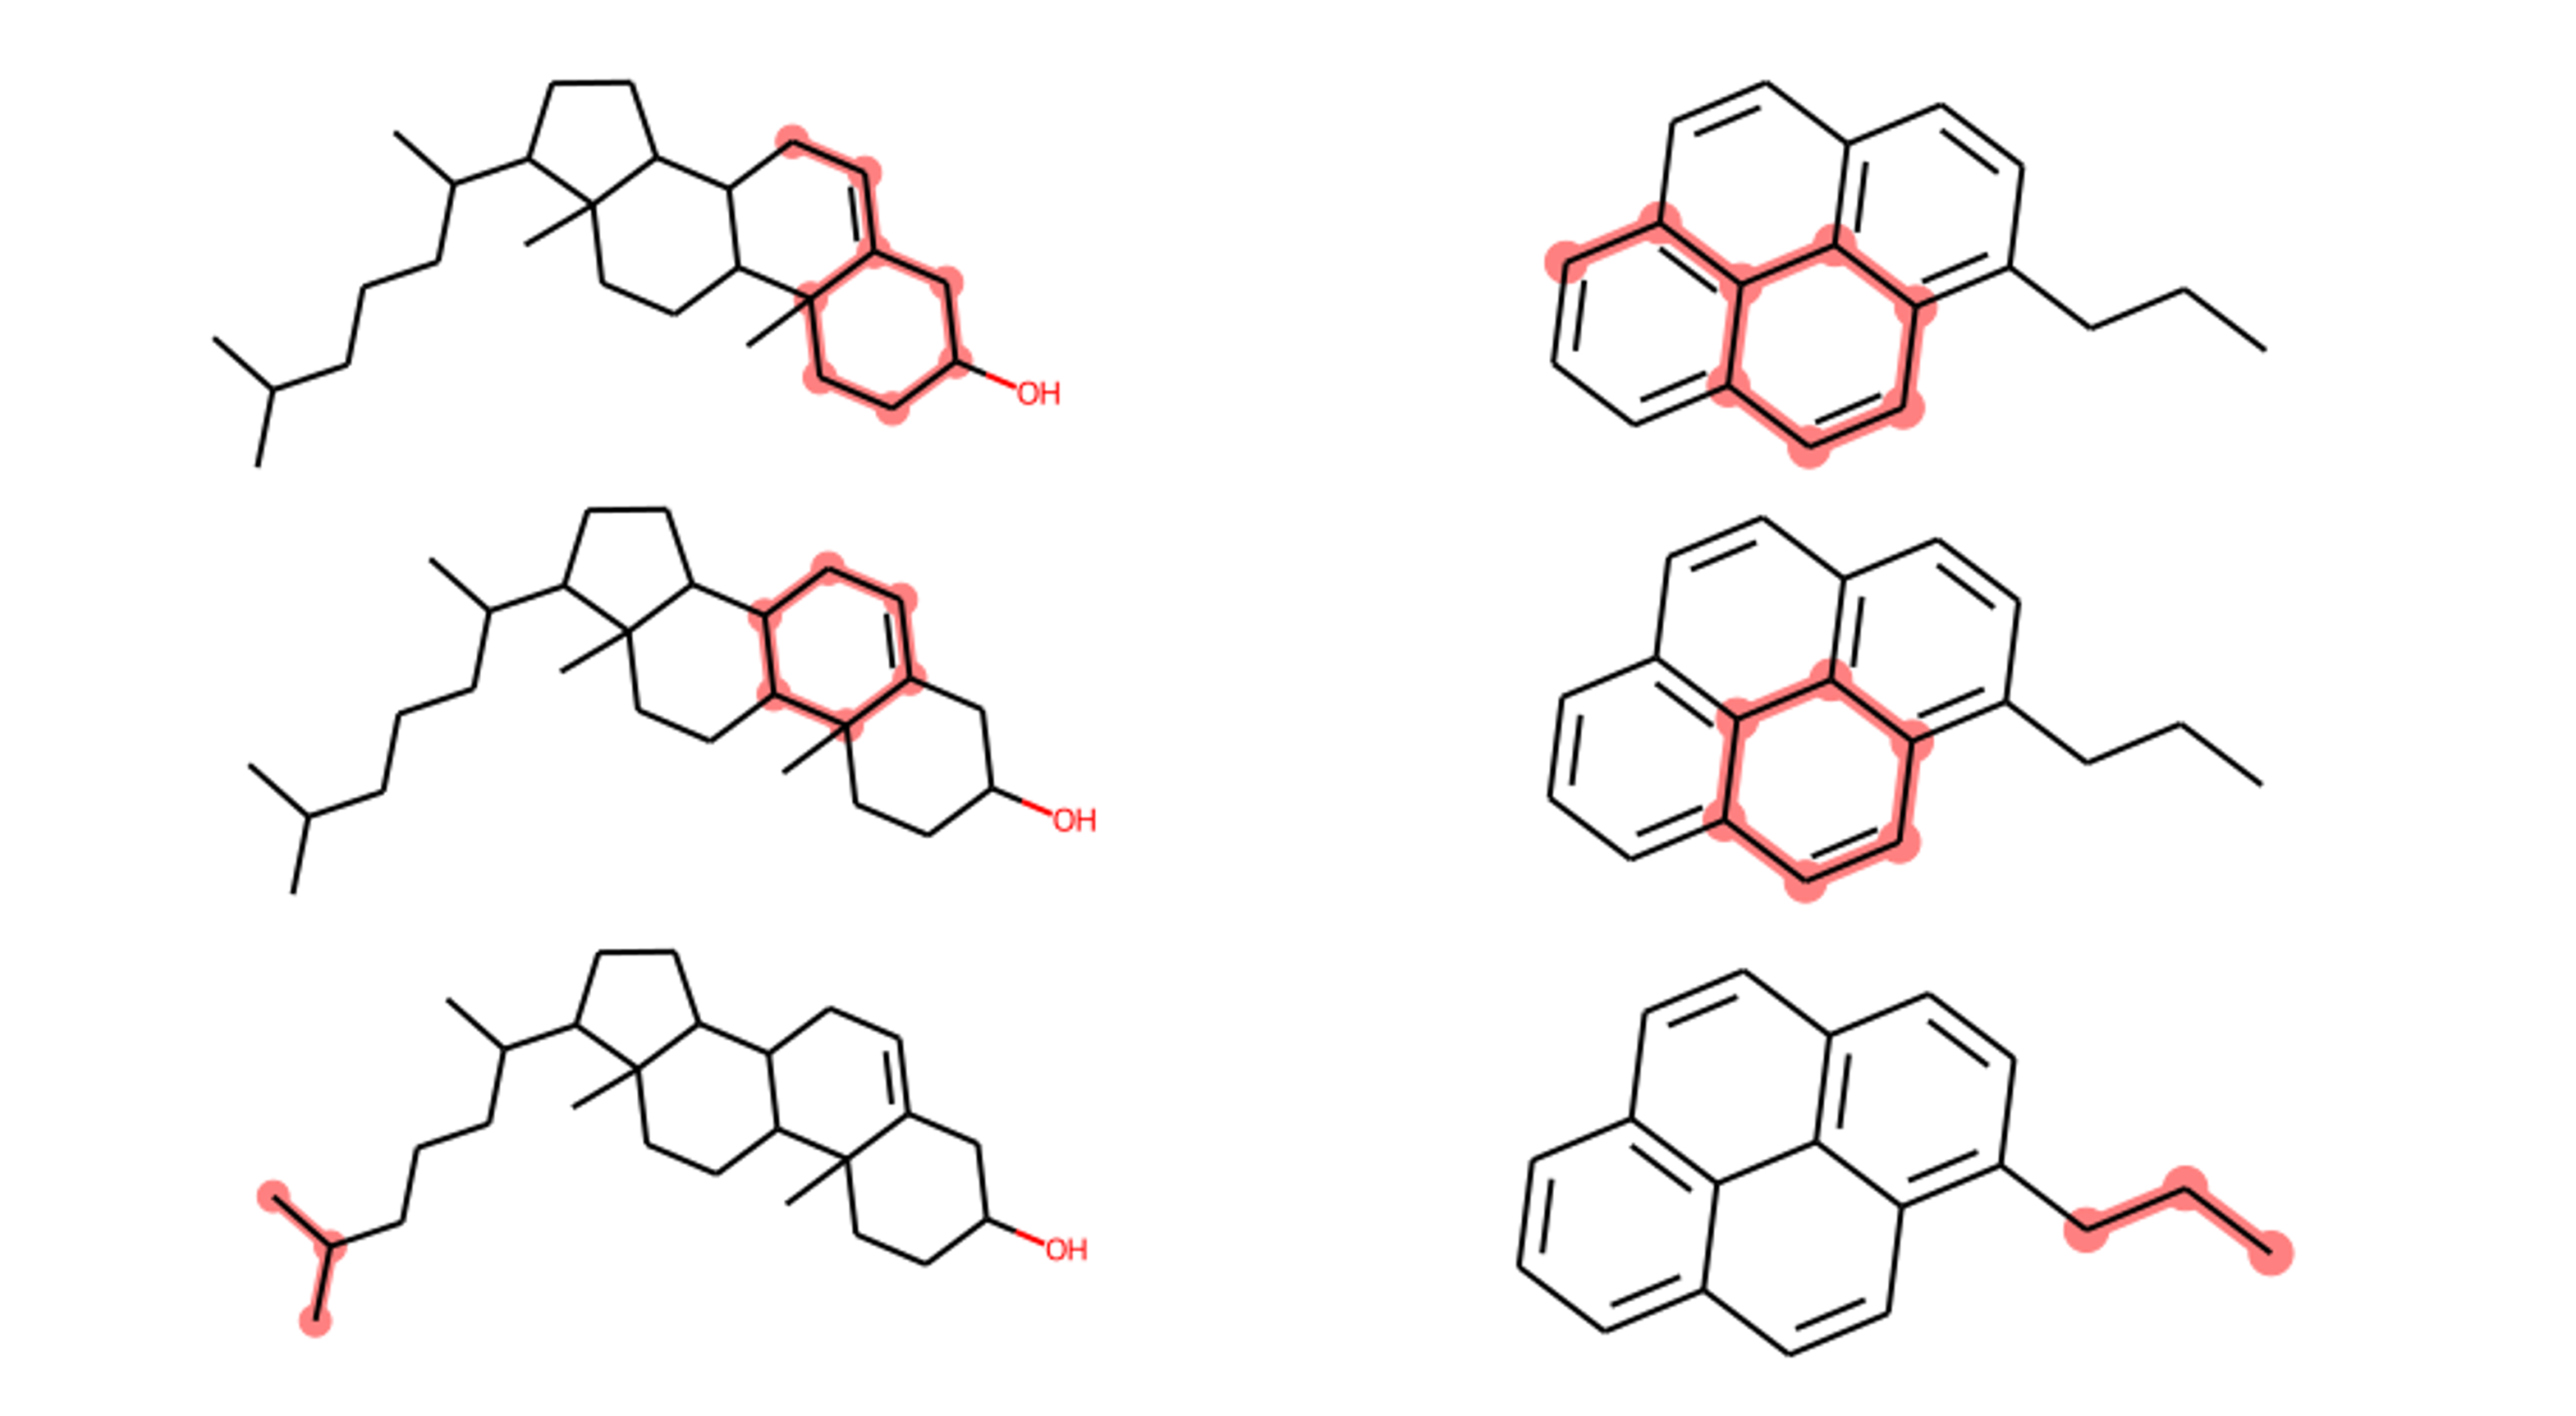
\includegraphics[scale=0.6]{cholesterol_pryenepropanoic_acid.png}
	
	\caption{common cores of cholesterol (left) and 1-pyrenepropanoic acid (right); upper row: CompleteRingsOnly = False; middle row: CompleteRingsOnly = True; lower row: iterative approach to obtain a valid {\trafo} common core}
	\label{fig:pyrene}
\end{figure}

If this is not the case, the rings that contain atoms which participate in the partial ring causing the invalid common core are removed from the representation used for creating the maximum common substructure and afterwards a new search for a valid common core is started. This procedure is repeated iteratively until a valid common core is found.
Of course, in the worst scenario, i.e. if both (non-identical) molecules only consist of ring-participating atoms, no valid common core is conceivable (and, given the total size of the molecules, the valid size can be very small). In general, if at least one of the molecules solely consists of a polycyclic compound without any functional groups etc., and the other one does not have exactly the same compound, no valid common core can exist. 
An – maybe rather contrived – example for such a pair of molecules and the construction of valid common core via the iterative approach is given in Fig. ~\ref{fig:pyrene}. One sees that even the usage of the ring-related parameters of Rdkit doesn't yield a valid common core, whereas the iterative approach gives the desired result.



\section{Graph algorithms}

Using NetworkX and Rdkit, the molecules and their common core are
represented as graphs (in which nodes indicate atoms and edges bonds
between them). The selection of the optimal mutation route can be
understood as a graph traversal problem in which the constraints mentioned
above are either implemented via the weights of the edges or sorting.
Hence the main task was to find suitable algorithms and graph initializations
to ensure an optimal processing of the mutation path.

Depth First Search (DFS) follows each chain of the graph as long as
possible, i.e. until a leaf node is reached. In contrast, Breadth
First Search (BFS) explores all chains simultaneously.\cite{Even.2012}
(Problems and differences of both algorithms are illustrated using
several examples below.)

In each of the algorithms implemented, the graph traversal starts
with the node which connects dummy region and common core as the root.
Shortest paths to all nodes of the dummy region are determined.

\begin{figure}

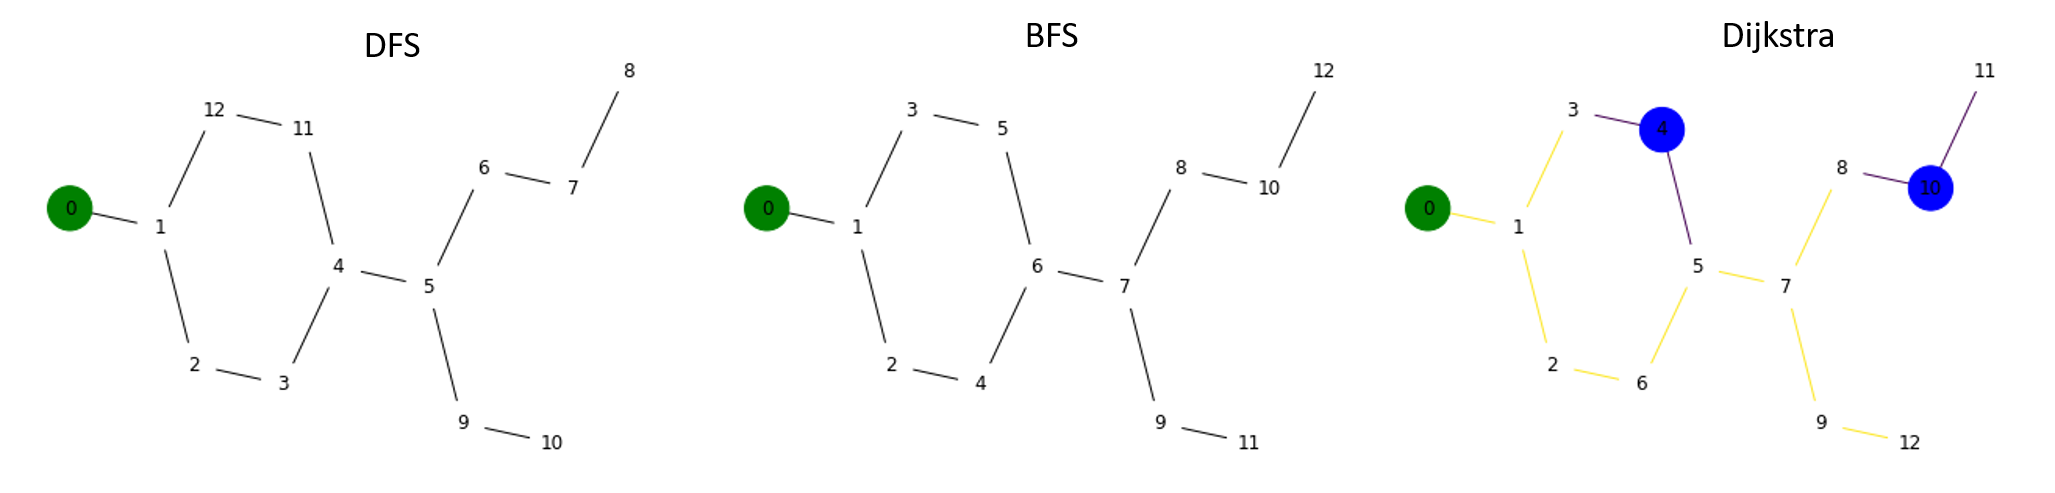
\includegraphics[scale=0.45]{dfs_bfs_dijkstra_comp1}\caption{Comparison of different graph traversal algorithms; green nodes represent the root atom, blue atoms (in the figure shown right) have increased weights; left: depth first
search; middle: breadth first search; right: Dijkstra algorithm, the
edges connecting blue colored nodes have increased weights leading
to a mutation route differing from BFS; the final processing of the
nodes happens in reversed order}

\end{figure}

As the longest shortest path pertains to the node which has the greatest
distance from the root (i.e. the atom with greatest distance from
the common core), the last element of the list returned by the search algorithm indicates the atoam which has to be removed first; hence, the list of mutations orders finally has to be reversed.

If weighted graphs are used, the Dijkstra algorithm can be applied.
It finds the shortest path between two nodes or between a root node
and all other nodes of the weighted graph (the weights indicate the
edge length from one node to the other one). For unweighted graphs
(or, equivalently, graphs with uniform weights), the Dijkstra algorithm
reduces to BFS. Fig. 4.3 shows the different routes for modified weights.
(In the test cases presented below, all graphs are initialized with uniformly weights.)

\section{Added functionality}

\subsection{Functions for creating mutation paths}

To use the newly implemented mutation algorithms, initially the graph
is given with weights stored in a dictionary. The simulations shown
below use uniform weights, however it is possible to modify these to
enforce a specific mutation route (e.g., accelerating or postponing
the exclusion of heteroatoms). 

The Dijkstra algorithm is implemented via the \texttt{single\_source\_dijkstra}-function
of NetworkX.

The core functionality is given by the mutation processing functions.
At the moment, three such functions are implemented, in addition to
the simple DFS-approach, which leads to undesired outcomes, in particular because often heavy atoms in neighborhood to the common core atoms are processed at the first steps of the graph algorithm as well as rings are opened early, but finally processed at a later stage (in a rather 'asymmetric' manner). These functions
can be further modified by passing arguments which activate some helper
functions (see below).

The four main functions for computing mutation routes are: 

\texttt{\_calculate\_order\_of\_LJ\_mutations:} naive DFS 

\texttt{\_calculate\_order\_of\_LJ\_mutations\_new:} BFS/Dijkstra-algorithm
applied once for route

\texttt{\_calculate\_order\_of\_LJ\_mutations\_new\_iter:} BFS/Dijkstra-algorithm
applied iteratively, i.e. after each removal of an atom 

\texttt{\_calculate\_order\_of\_LJ\_mutations\_new\_iter\_change:}
works iteratively, i.e. after each removal of an atom, the algorithm/routine for the next step is chosen depending on current state

\texttt{\_calculate\_order\_of\_LJ\_mutations }was already present in {\trafo}, but computes defective mutation routes and hence
should only be used for test purposes. The other three algorithms
are new and, in any case, resolve most of the problems of the earlier
algorithm (especially isolated removal of ring atoms).

Helper functions like cycle\_checks carry out tasks to ensure the
desired mutation route, e.g. count the number of cycles an atom participates
in. Further features of all algorithms are 'preferential removal',
i.e. if two atoms would have the same priority (given by the current
weight) for the next mutation step, the weight of the atom which is
next to an already removed atom is updated so that this atom is excluded
next.

\texttt{cycle\_checks(G)}: this function checks which atoms participate
in how many cycles/rings and returns a dictionary with the atoms as
key and the number of rings the atom is participating in as value
and a dictionary with the degree (i.e. number of edges) of each atom
node. It is currently used in \texttt{\_calculate\_order\_of\_LJ\_mutations\_new}
(via the \texttt{change\_route\_cycles}-function).

\texttt{change\_route\_cycles}(route, cycledict, degreedict, weightdict,
G): this function is used in \texttt{\_calculate\_order\_of\_LJ\_mutations\_new}
and sorts nodes according to degree, cycle participation and information
about the nodes which have been removed immediately before. The preliminary mutation
path is sorted using cycle and degree dictionary. If nodes have same
weight (i.e. distance from root), the node participating in more cycles
is removed later if nodes have same the weight (i.e. distance from root)
and same cycle participation number, the node which has more neighbours
already removed is removed earlier

\texttt{cycle\_checks\_nx}(G): This function modifies the weight of
the graph, nodes participating in many cycles get lower weight. It
is currently used in 
\texttt{\_calculate\_order\_of\_LJ\_mutations\_new\_iter} and \texttt{...\_new\_iter\_change.} It returns a nx-graph-object
with updated weights (according to cycle participation of the atom).

\texttt{order\_checks\_nx}(G, removearray, G\_total): This function
performs the 'preferential removal', if a node is connected to the
node removed in the last step, its weight get a small increase so
that the removal of this node is prioritized. It is currently used
in\texttt{ \_calculate\_order\_of\_LJ\_mutations\_new\_iter} and returns
a nx-graph-object with updated weights.

If the cyclecheck-argument of the new mutation algorithms is True,
updates are updated according to cycle participation (as the systematic
processing of ring structures is one of the central goals, this argument
should always be set to True, except for comparison and test purposes).
If in the case of \texttt{\_calculate\_order\_of\_LJ\_mutations\_new
and \_calculate\_order\_of\_LJ\_mutations\_new\_iter} also ordercycles
or ordercheck, respectively, is set to True, weight updating according
to preferential removal decides that the node in which neighbourhood
nodes already have been turned off is removed next if there is no
possibility to decide between two nodes - i.e. the weight of both
would be exactly the same.

In each algorithm, all nodes of the graph (i.e. atoms) are usually
initialized with the same weight (e.g. 5). Alternatively, the user
could also pass an individual dictionary with different weights for
each atom type.

The BFS- / Dijkstra-algorithm starting from the node connecting common
core and dummy region is applied via the NetworkX-function \texttt{single\_source\_dijkstra}
which determines the path length of all dummy nodes to the root.

The main difference between these algorithms is that in \texttt{\_calculate\_order\_of\_LJ\_mutations\_new\_iter}
and \texttt{...\_iter\_change} the graph traversal part performed
using the Dijkstra algorithm is applied after each exclusion step; i.e. $n!$ atoms are visited instead of $n$; even for large molecules the additional computational cost is negligible, in particular in comparison
to the computational time needed for the search of the common core.
The advantage of the iterated version is that after each mutation step weights can be
updated or even the search algorithm can be modified. 

This feature allows for different mutation strategies depending
on the current state. Such an approach is demonstrated in \texttt{\_calculate\_order\_of\_LJ\_mutations\_new\_iter\_change}.
In contrast to the other algorithms, the algorithm processes information
if the last removed node was part of a chain or a cycle. Depending
on the state, the chain or cycle is processed fully before the algorithm
moves on to other parts of the molecule. Fig. 4.5 demonstrates the difference between the two versions of the iterated algorithm.
Whereas in the non-iterated algorithm the found mutation route has to be reversed (since the atom node with the highest distance from the root is the first which has to be turned off), in the iterated versions at each iteration the node with the highest distance is added to an array which determines the final mutation route.

The computed mutation routes can be visualized directly via Rdkit. 
The route is represented by a colour gradient used for the atoms involved
in the mutation process (\texttt{\_show\_common\_core\_gradient}). By default, the color spectrum ranges from red to green; the first atom to be removed is colored red, the last green.

Furthermore, an animated 3D-visualization of the mutation process
is implemented using py3Dmol (\texttt{animated\_visualization\_3d\_v2})\cite{key-4}. 

\begin{figure}
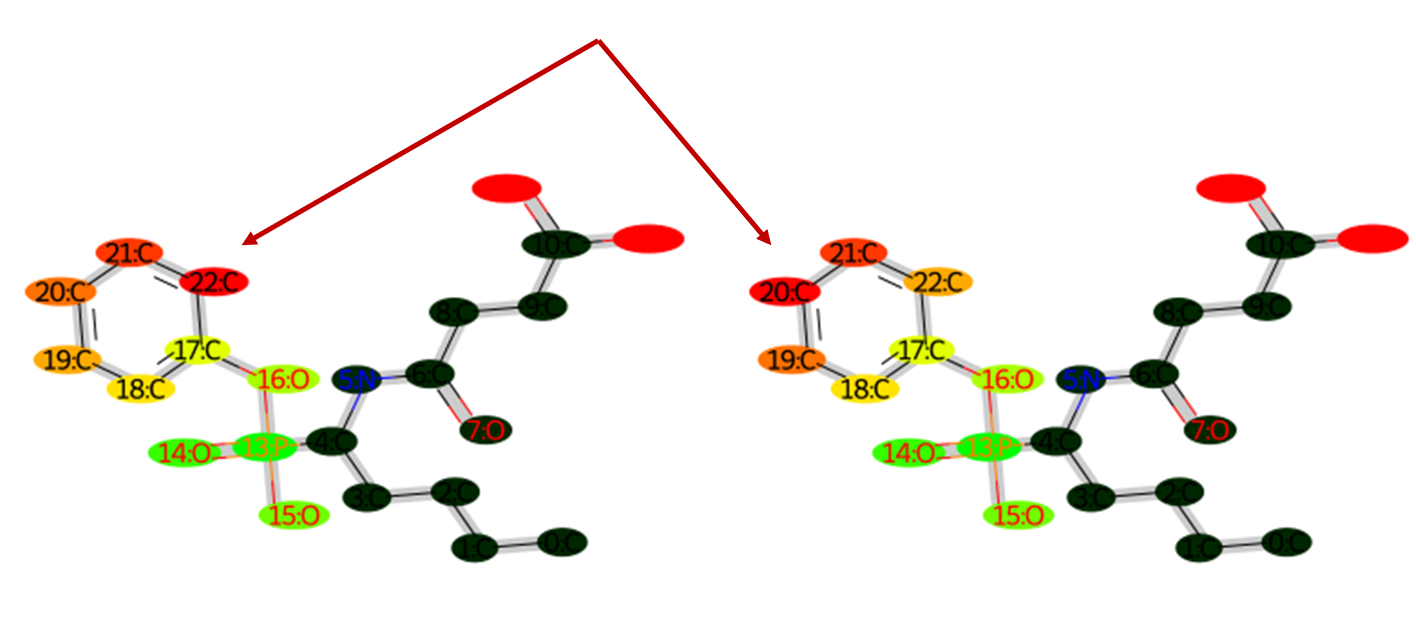
\includegraphics[scale=1.4]{simple_ring_exampledfs.png}

\caption{comparison of typical DFS- and BFS-mutation route for a single ring structure; left: DFS-algorithm; right: BFS-algorithm; in all depictions of mutation routes the common core is shown in dark, the color gradient starts at red indicating the atom first to be removed and ends at green; DFS
starts at carbon 22 and thus ring breakage gives rise to one long
chain which is processed subsequently, whereas BFS starts at carbon
22 and the two emerging chains are processed in a symmetric fashion
}

\end{figure}


\subsection{Processing of hydrogen atoms}

\begin{figure}
	
	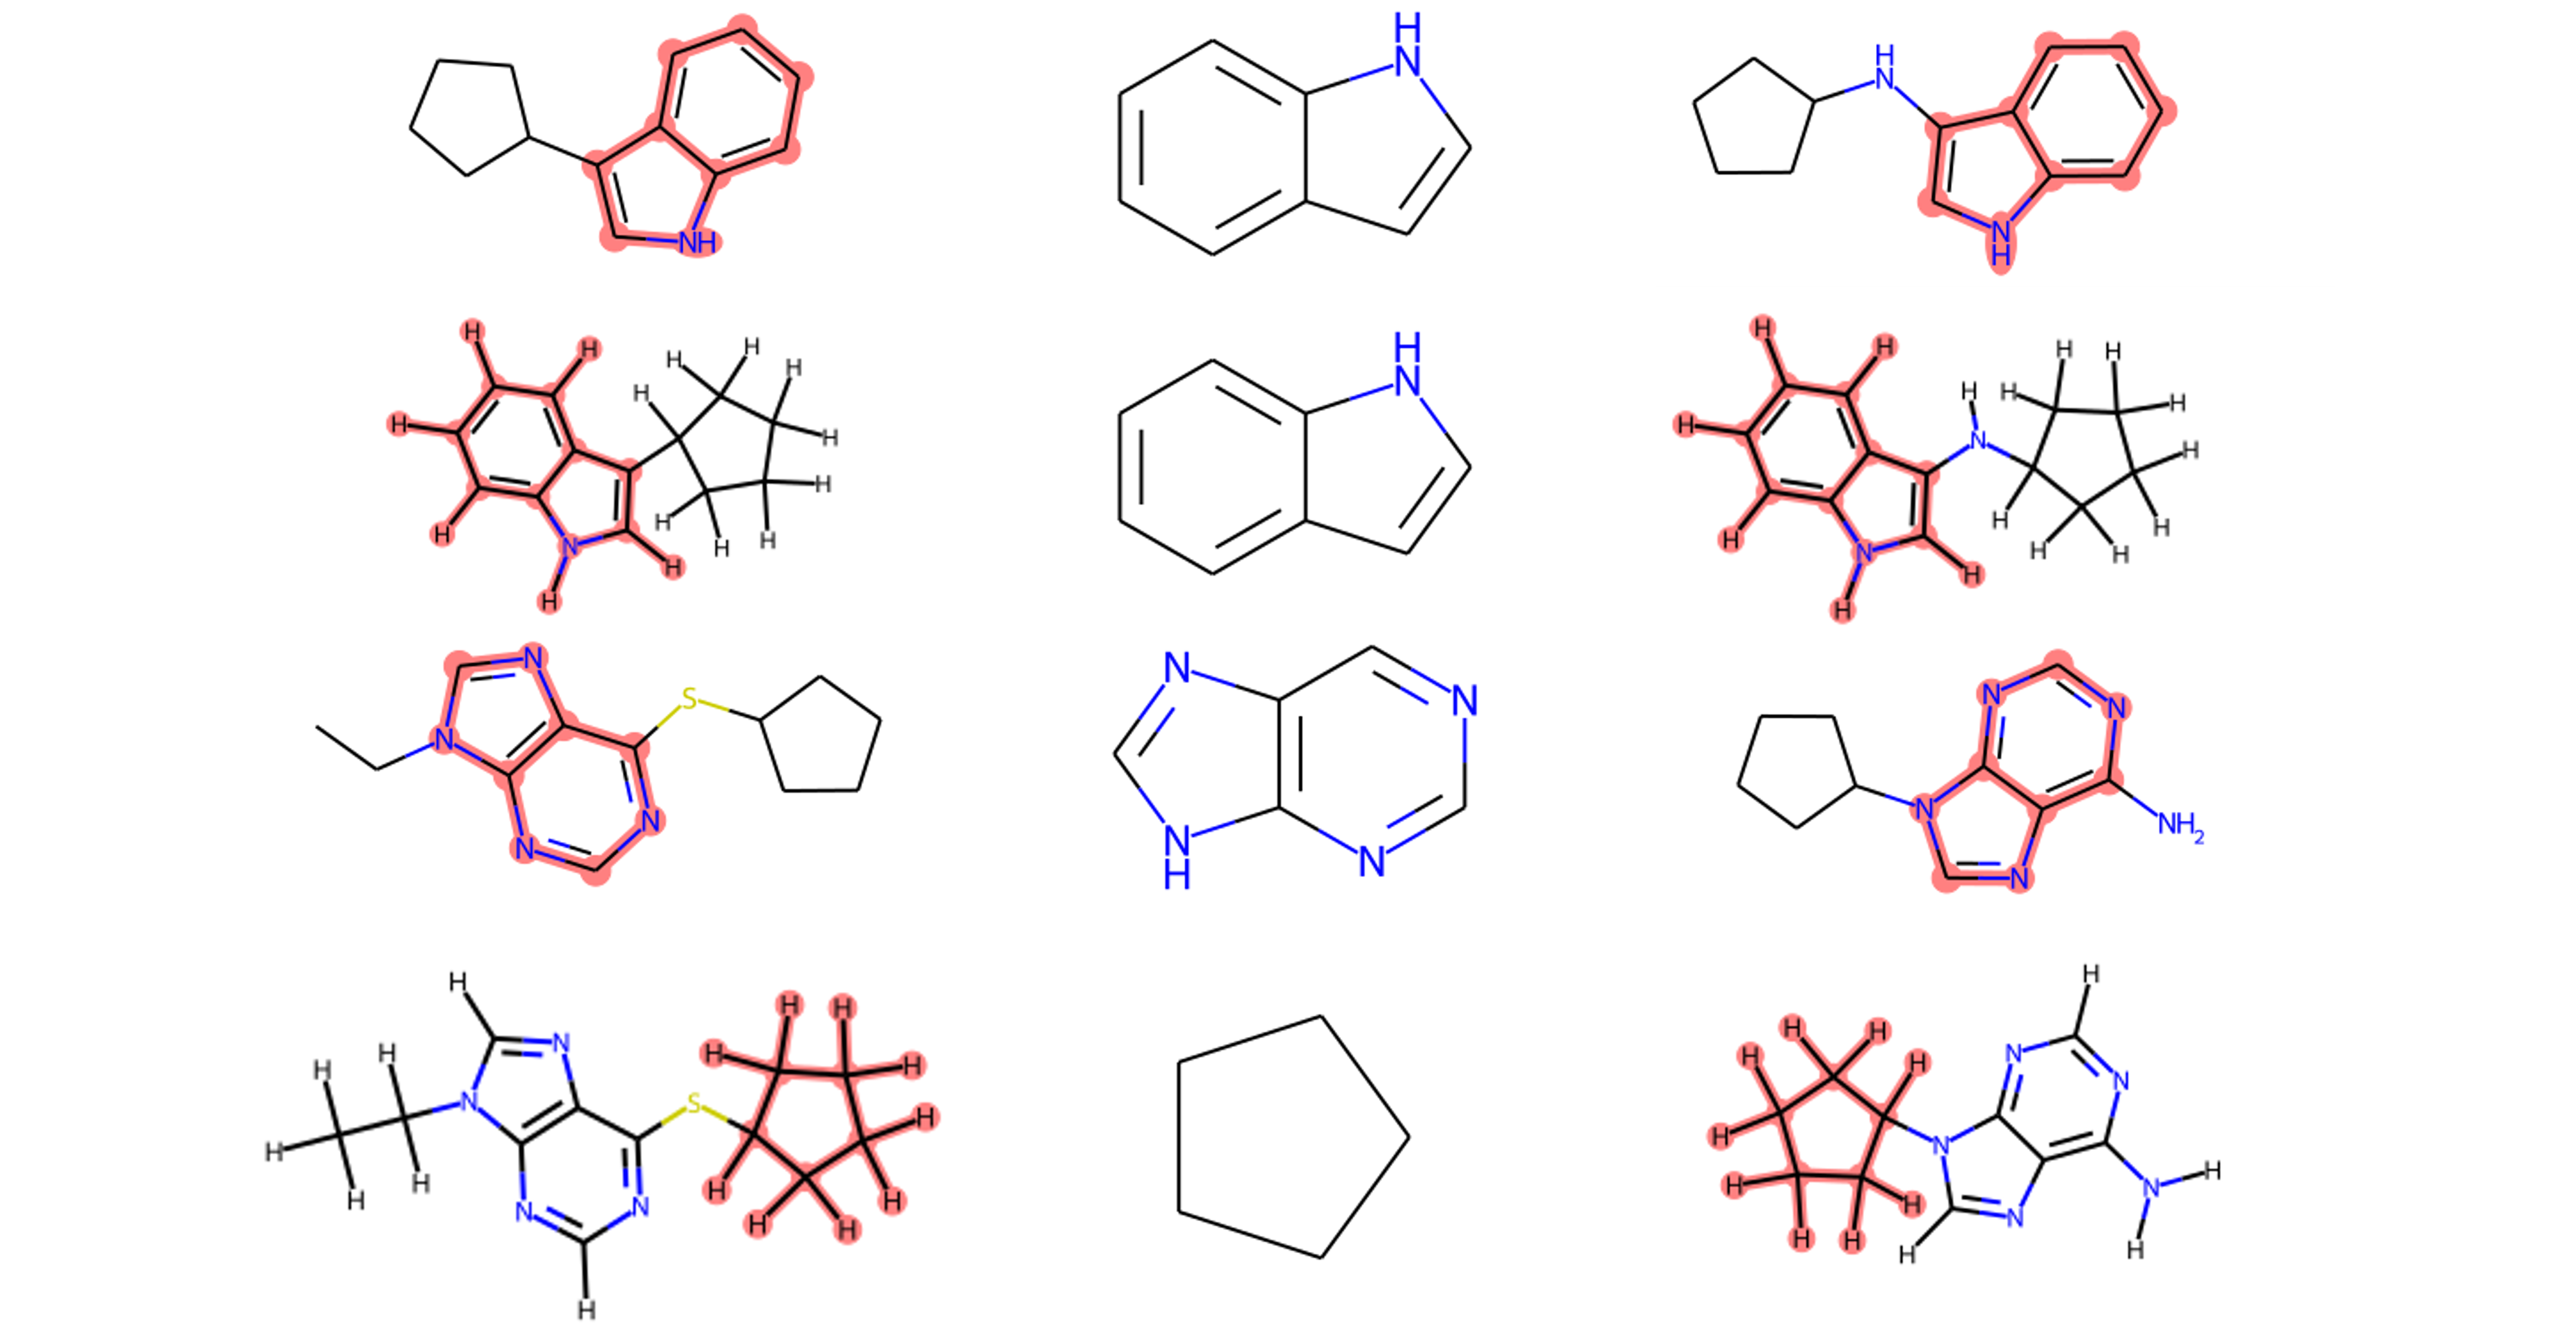
\includegraphics[scale=0.35]{hydrogens_plus_minus}
	\caption{These examples demonstrate that the addition of hydrogens can influence the construction of the common core; left: molecule 1; middle: common core; right: molecule 2; in the representations of the full molecule, the common cores are marked in red; the first
		and the last two rows show the same molecules, in the upper row without,
		in the lower with hydrogens, in case of the lower molecule combination
		the common core changes when hydrogens are added to the Rdkit-molecule
		representation }
		\label{fig:hydrogen_effect}
	\end{figure}


As fig. \ref{fig:hydrogen_effect} indicates, the presence of hydrogens can influence the common core generation dramatically. In particular, the maximum common substructure for a molecule representation with hydrogens can encompass less heavy, i.e. non-hydrogen, atoms than the substructure for a representation with hydrogens removed (although, including the hydrogens, the total number of atoms is higher in the first case). Hence it is crucial to determine the common core for molecule representations without hydrogens. Since hydrogen atoms are turned off in an extra step en bloc during the {\trafo} workflow, the mutation route algorithm should not take hydrogens into account nor must the common core be generated for a molecule representation containing hydrogens.
Nonetheless, it is necessary that the molecule representations processed in Tranformato contain all hydrogens in explicit form because the indices of these atoms in the underlying data structures are used in some steps, e.g. for scaling the van-der-Waals interactions of the hydrogen atoms to zero.
This problem was solved by removing and adding hydrogens appropriately.
In a first step, the {\trafo} function determining the common core (\texttt{\_find\_mcs} in mutate.py) had to be modified. To obtain the desired common core but retain the {\trafo} workflow, the following scheme was implemented:
A deep copy of both molecules is created. The hydrogens of these copies are removed and afterwards their common core is computed. For both molecules, the indices of the atoms corresponding to the common core are determined. Finally, it is checked for each common core atom of both molecules whether hydrogen atoms are in its neighbourhood. If such hydrogens are found, their indices are added to the lists of common core atoms. These lists of atoms including hydrogens are stored for both molecules and the function returns the maximum common substructure (determined for the molecules without hydrogens).
Thus the procedure yields the necessary output for further processing in {\trafo}: The molecule representations and lists of common core atoms for both of the molecules include hydrogens, but the maximum common substructure giving rise to the common core is computed only for the heavy atoms.
Similarly, the functions for computing the mutation routes had to be adapted for input molecules containing hydrogens. By default, a helper function removes the hydrogens from the graph representation as well as the corresponding indices from the list with the atoms of the dummy regions before the mutation algorithms are applied. Afterwards, the hydrogen atoms adjacent to common core heavy atoms are added to the common core.
A special problem occurs for molecule pairs with switching 'X'-atom; fig. \ref{fig:pyrrolidinindole} shows 2-/7-pyrrolidinindole as example. It is necessary that a further dummy region emerges which consists solely of one hydrogen atom because otherwise the common cores would have a different number of atoms. It depicts a correct common core for both molecules; one should note the hydrogen atom which is not part of the common core. If, however, the common core is generated without hydrogens, the information which of the hydrogens turns into a dummy region is lost.
It has to be stressed again that the presence of these hydrogen dummy regions does not affect the mutation steps, but is nonetheless crucial for the internal {\trafo} workflow. However, there is a straightforward way to circumvent this problem: From the substructure matches the mapping between the common core atoms of each molecule can be read off. It is counted for each heavy common core atom how many hydrogens are connected to it. Finally, the minimum number of hydrogens is added to the common core. (In the case of 2-/7-pyrrolidinindole, this means that for each common core atom one hydrogen is added, except for the 2- and 7- position, because for these positions in one molecule no hydrogen is connected).
In this context, also the difficulty that there are possibly many substructure matches has to be mentioned.
It is even possible that substructure matches differ solely with respect to hydrogens. For this case, a parameter was added to the function which searches for the maximum common substructure. If \texttt{iterate\_over\_matches} is set to true, one of the substructure matches with most hydrogens, i.e. the biggest possible substructure, is selected. Fig. \ref{fig:neopentan} shows two common cores only differing in the number of hydrogens.



\begin{figure}
	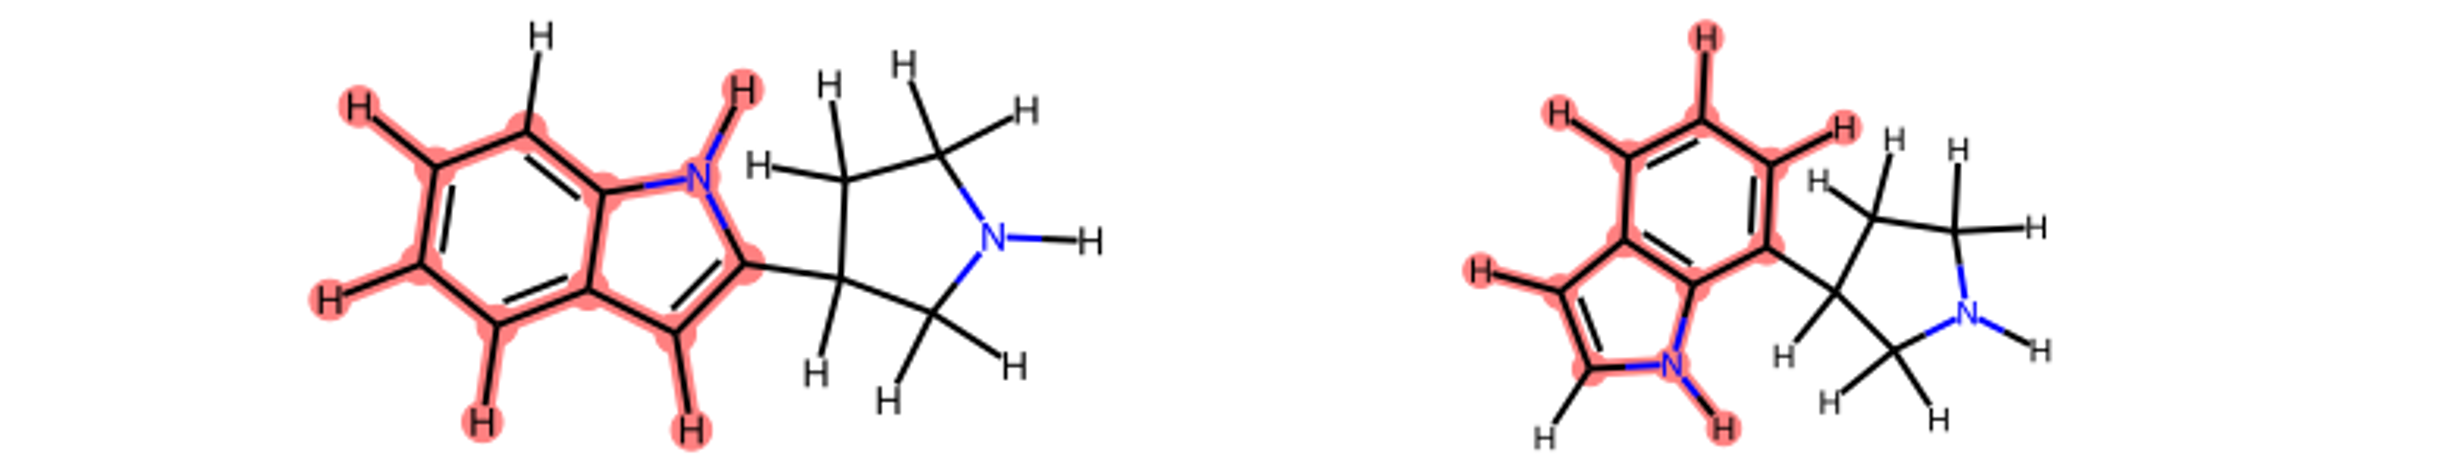
\includegraphics[scale=0.8]{pyrrolidinindole}
	
	\caption{
		left: 2-pyrrolidinindole; right: 7-pyrrolidinindole; 
		one of the hydrogens - exactly this hydrogen which becomes the junction 'X'-atom - is not part of the common core}
	\label{fig:pyrrolidinindole}
\end{figure}


\begin{figure}
	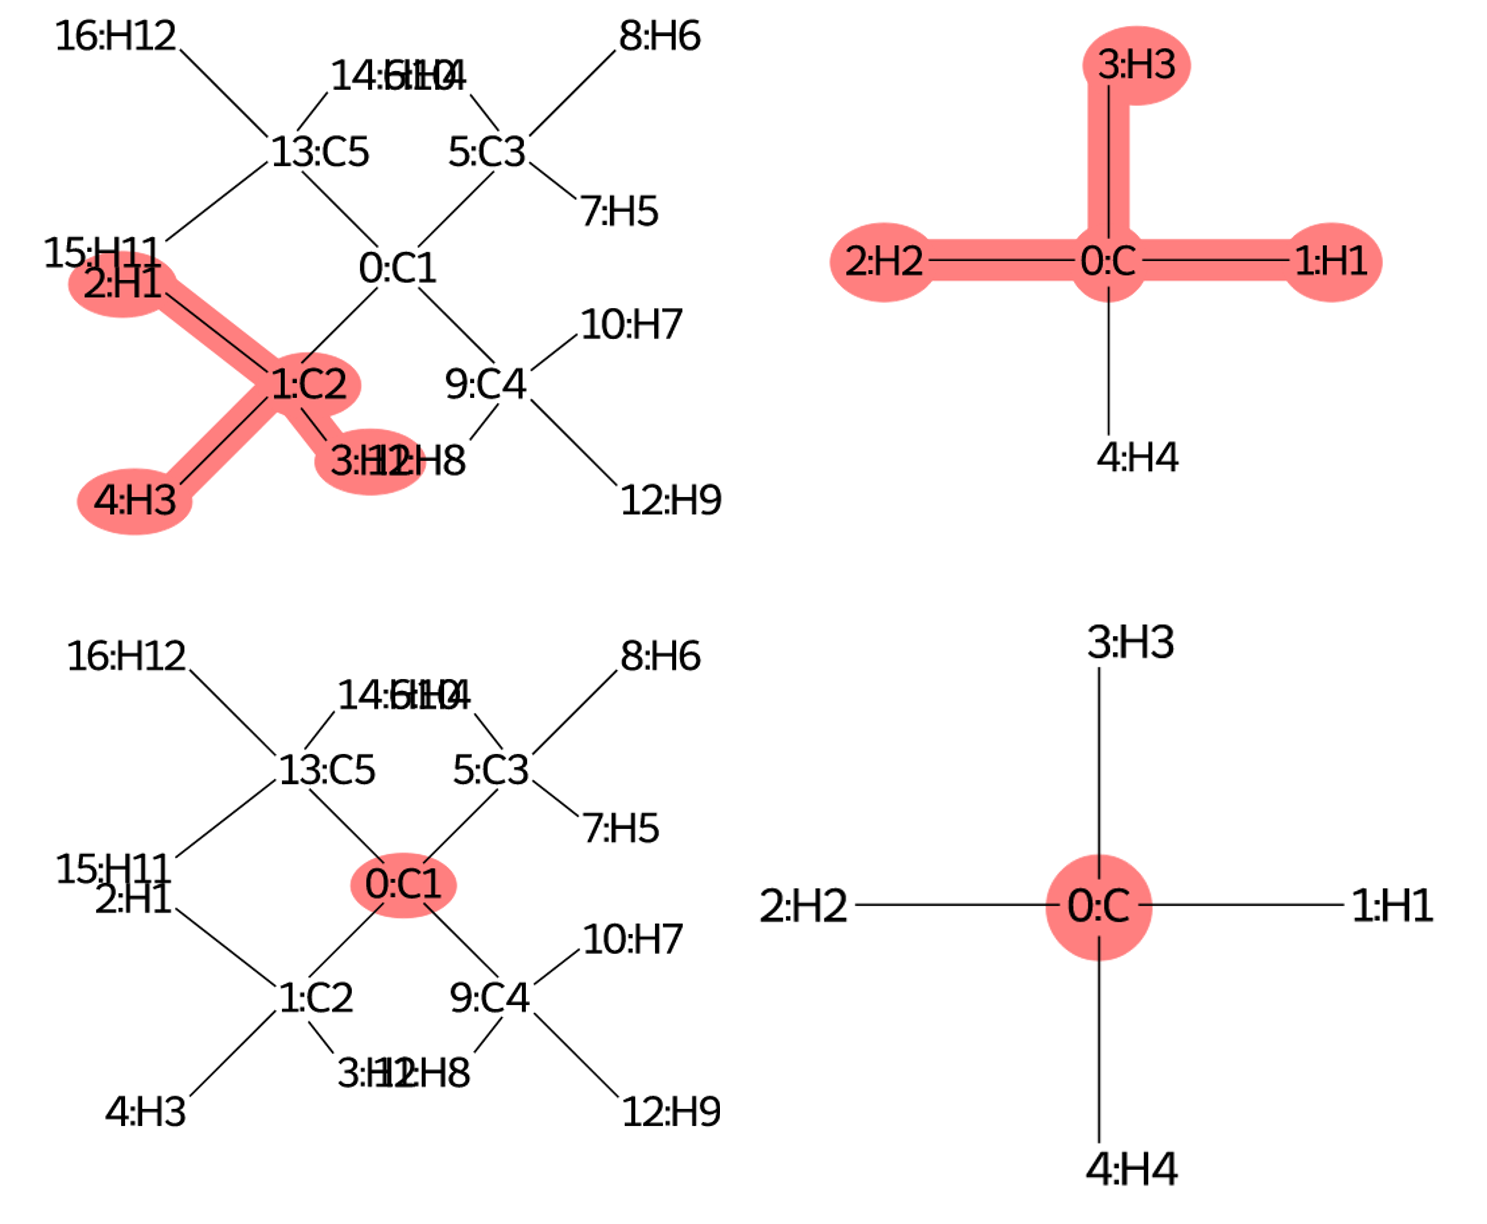
\includegraphics[scale=1.0]{neopentan}
	
	\caption{neopentan/methane common cores; upper row: common cores maximizing the number of atoms including hydrogens; lower row: common cores without considering hydrogens}
		\label{fig:neopentan}
\end{figure}



\subsection{Examples for processing molecules}

\begin{figure}
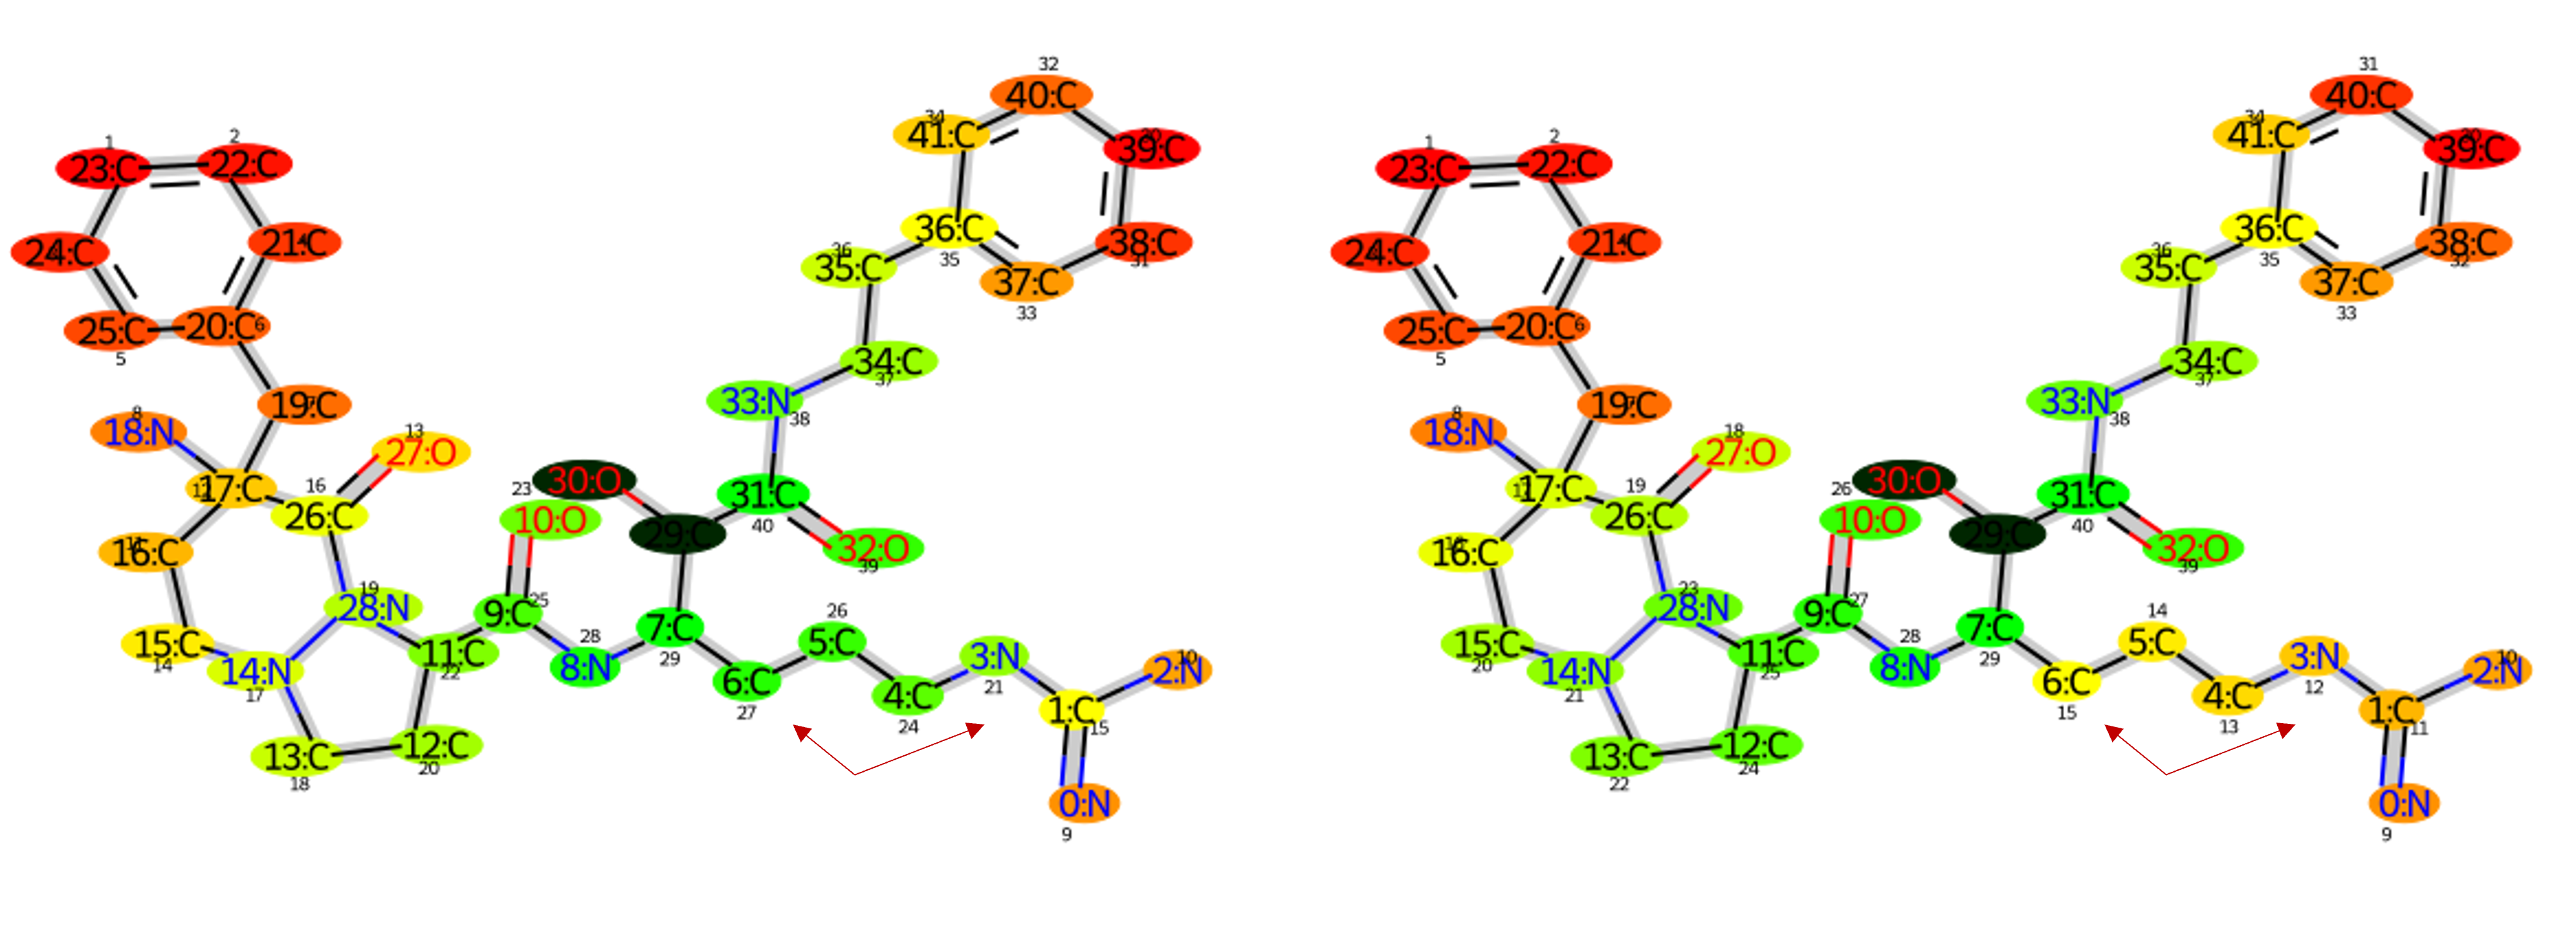
\includegraphics[scale=0.5]{iter_iter_change_1a5g_1}

\caption{Example for the differences between iter- and iter\_change-algorithm;
left: iter; right: iter-change; iter-change processes all atoms within
a chain or a ring at once (if possible) before switching to other
parts of the molecule}
\end{figure}

In the current version of {\trafo}, one suboptimal route finding algorithm using DFS and several new versions based on BFS are implemented.
For single rings, BFS (or, in the case of different weights for various atom types, the Dijkstra algorithm) automatically processes the atoms in the most symmetric way starting at the atom with the highest distance from the root (fig 4.4).
In more complex molecules, the systematic exploration of chains in
depth first search inevitably leads to big local gaps in processing
of the molecules. Fig. 4.6 shows this problem for a benzol ring which
is directly attached to the common core. As DFS goes along one path
until the end, i.e. until a leaf node is reached, only four atoms of the
ring are visited at the beginning, whereas the remaining two are explored
last. Therefore, these two atoms are turned off first, but then the
algorithm continues at a wholly different location and the remaining
ring atoms persist in the system until the end of the mutation process.
In this case, BFS automatically produces the desired result. 

Similarly, in fig. 4.7 one atom of the ring (marked by the red circle)
is omitted in the first exploration using DFS.

More complex ring structures exacerbate the problems. Fig. 4.8 shows that also the processing of substituents is affected.

Multiple rings pose special difficulties for the mutation algorithms because
the processing of one of the rings can easily led to gaps in the adjacent
ones. Fig. 4.9 and 4.10 show that using DFS aggravated problems occur.
As in the case of one ring, the exploration route implies that one
of the rings is opened in a way that it gives rise to a lengthy chain.
However, it can even happen that the atom explored atom participates
even in two or multiple rings, so that both ring structures are opened
and teared apart (fig. 4.9). Alternatively, one half of each of the
rings is turned off first (fig. 4.10). 

\begin{figure}
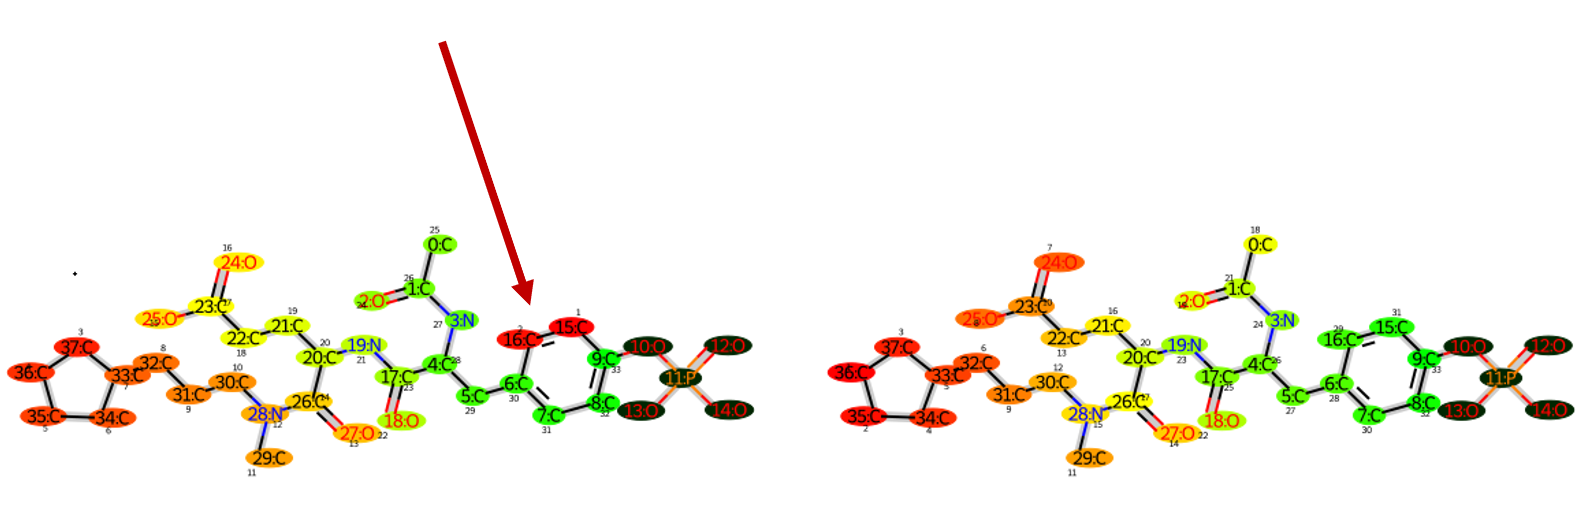
\includegraphics[scale=1.5]{simple_ring_exampledfs2}\caption{left: DFS-algorithm; right: BFS-algorithm; common core in dark; the
red arrow indicates the undesired processing of the ring atoms}

\end{figure}

\begin{figure}
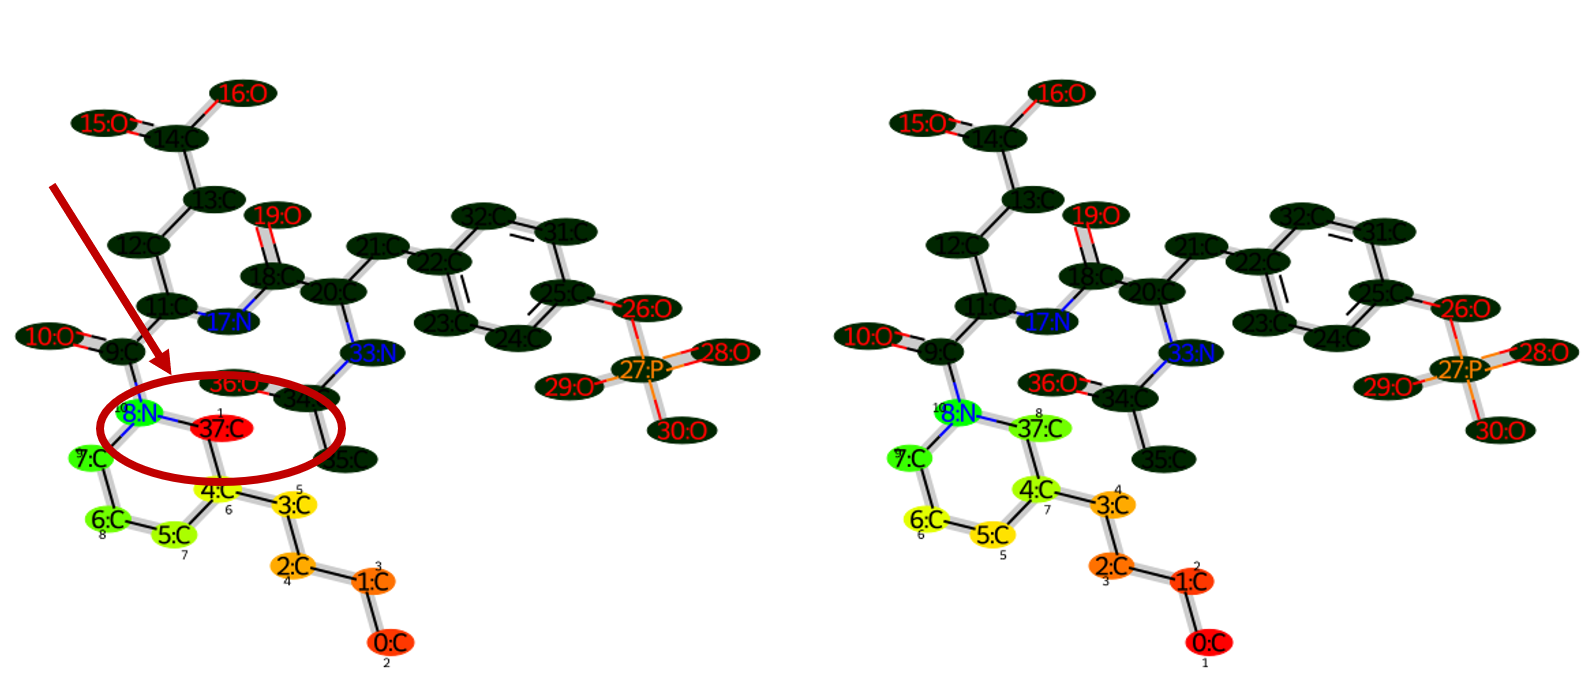
\includegraphics[scale=1.3]{simple_ring_exampledfs3}\caption{left: DFS-algorithm; right: BFS-algorithm; common core in dark; the
red arrow and circle indicates the undesired processing of the ring
atoms}

\end{figure}
\begin{figure}

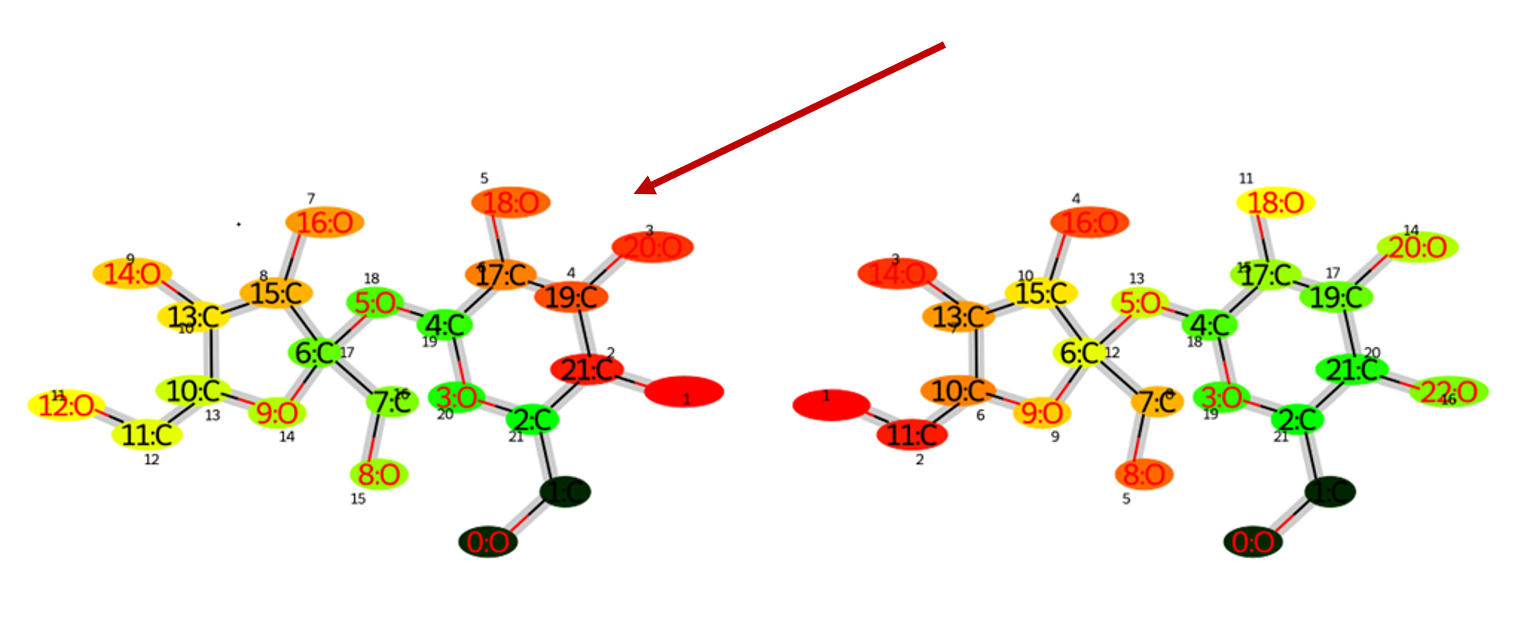
\includegraphics[scale=0.5]{simple_ring_exampledfs4}\caption{left: DFS-algorithm; right: BFS-algorithm; common core in dark; the
red arrow indicates the undesired processing of the ring atoms}

\end{figure}

\begin{figure}

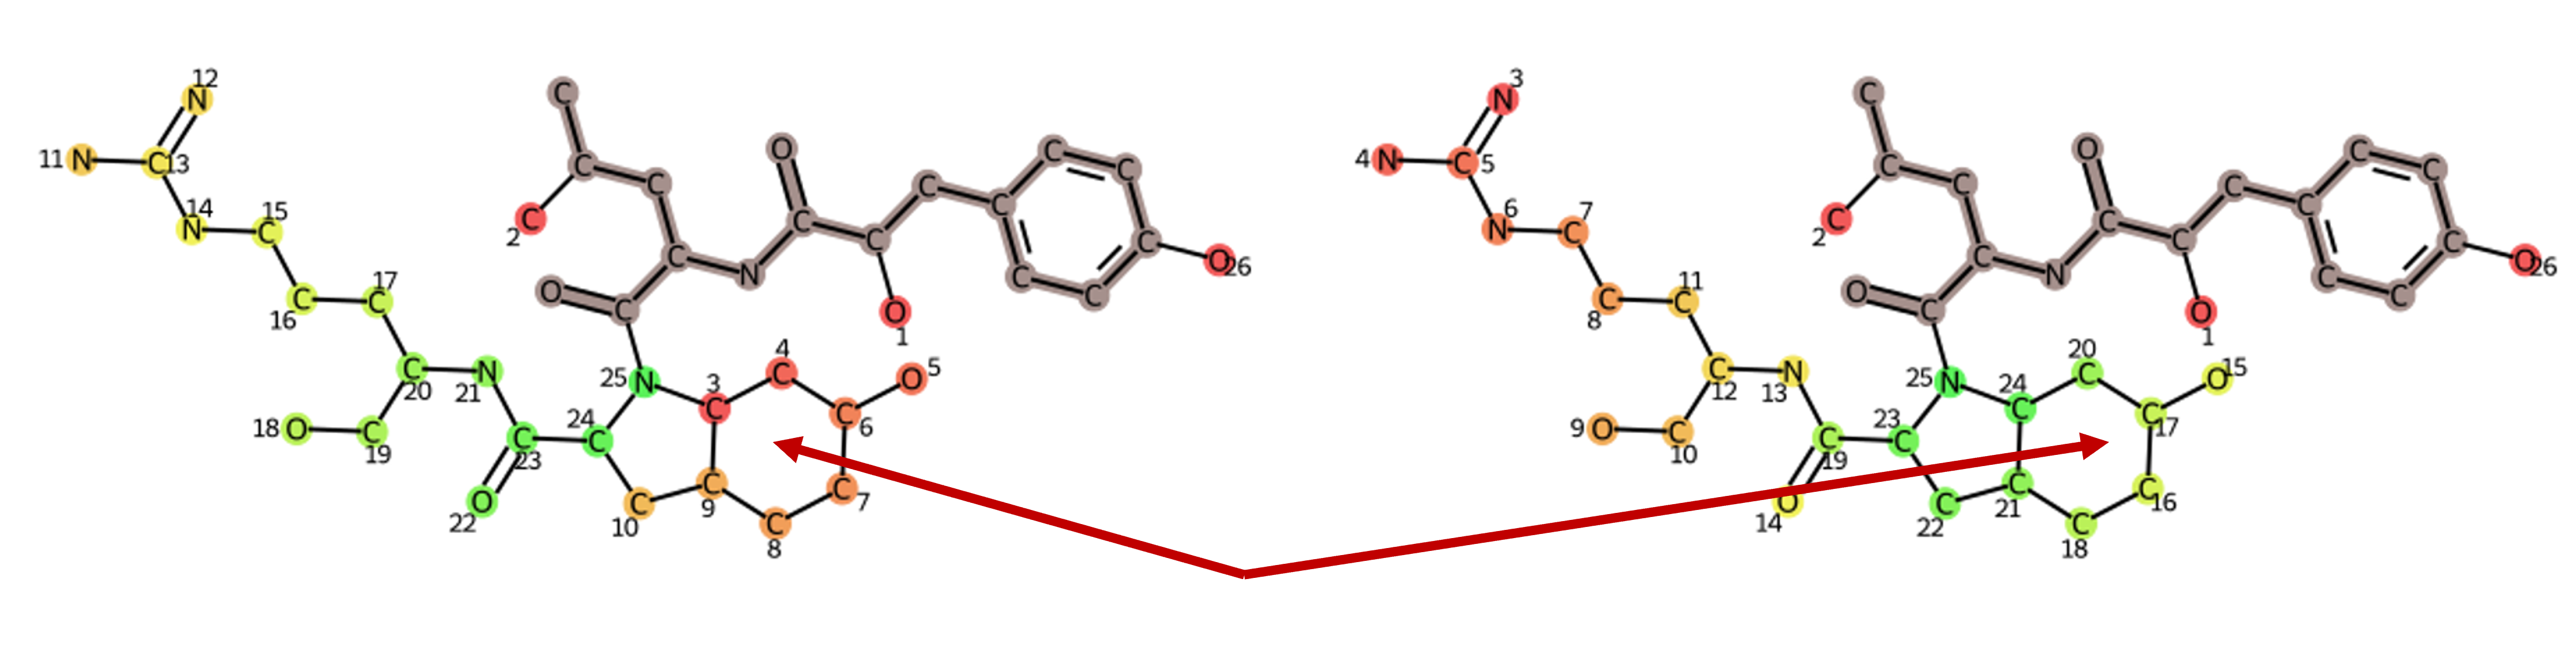
\includegraphics[scale=0.5]{2ring_example}\caption{left: DFS-algorithm; right: BFS-algorithm; common core in dark; the
red arrow indicates the undesired processing of the ring atoms}

\end{figure}

\begin{figure}

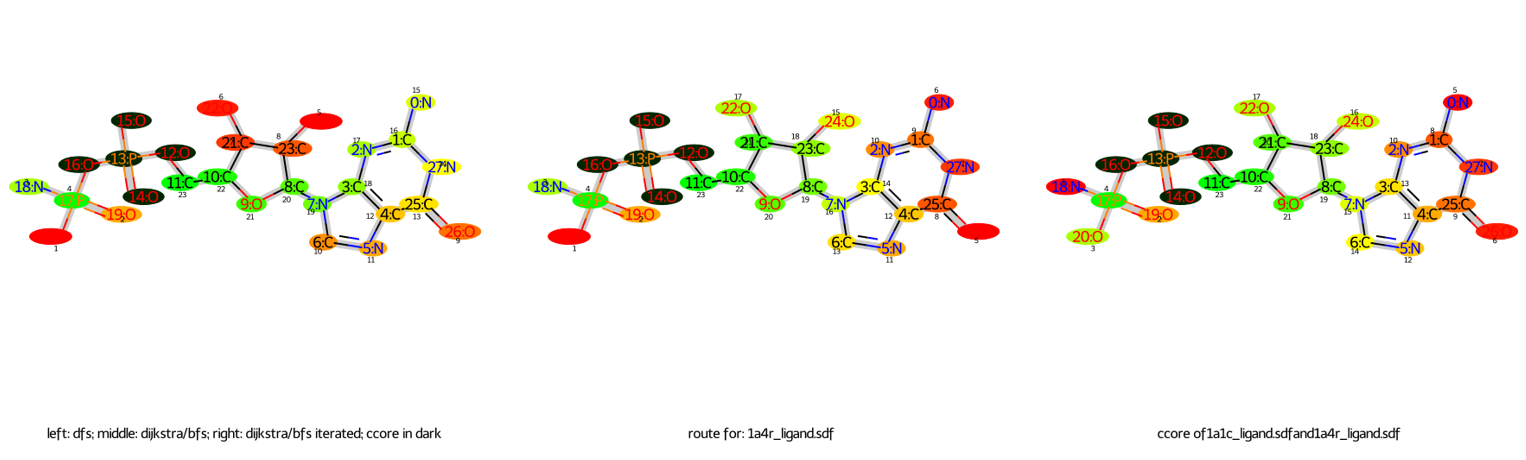
\includegraphics[scale=0.5]{2ring_example2}\caption{left: DFS-algorithm; right: BFS-algorithm; common core in dark}

\end{figure}
